\documentclass{article}
\usepackage[utf8]{inputenc}
\usepackage{graphicx}

\title{Analisi della caratteristica I-V di un diodo}
\author{Francesco Pio Merafina, Onofrio Davide Caputo, Alessandro Lamesta}

\begin{document}
\maketitle
\section{Abstract:}
Lo scopo dell'esperienza consiste nel verificare se effettivamente la legge di Schokley è in grado di descrivere il comportamento di un diodo. Per fare ciò è stato costruito un circuito che lavorasse in corrente continua e dal quale abbiamo prelevato la corrente e la tensione del diodo.
~
\section{Cenni teorici:}
Il diodo è definito come giunzione p-n; ovvero un cristallo di silicio che è un atomo tetravalente diviso in due regioni una drogata con atomi trivalenti, cioè la p, ed una drogata con atomi pentavalenti; cioè la n. Questa composizione ci permette di avere, una volta che colleghiamo il diodo ad un generatore di tensione, di avere la seguente caratteristica I-V detta legge di Shockley:
\begin{equation}
    I_d=I_0(exp(V_d/V_t)-1)
\end{equation}
I parametri dell'equazione sono i seguenti:
\begin{itemize}
    \item I$_{d}$=corrente nel diodo
    \item I$_{0}$=corrente di saturazione
    \item V$_{d}$=tensione ai capi del diodo
    \item V$_{t}$=tensione termica
\end{itemize}
La corrente di saturazione e la tensione termica sono caratteristiche intrinseche del diodo, dipendono dal procedimento di costruzione, e la loro modellizzazione teorica si può ricavare partendo dalla formazione di flussi di elettroni o lacune a causa della disomogeneità della distribuzione di cariche.
~
\section{Strumentazione:}
La strumentazione utilizzata per l'esperienza consiste in:
\begin{itemize}
    \item -Diodo
    \item -Resistenza di protezione di circa 100 $\Omega$ con una tolleranza del 5%
    \item -Multimetro digitale usato come voltmetro
    \item -Amperometro analoigico
    \item -Generatore di tensione
\end{itemize}
il tutto è stato montato su una scheda millefori usando dello stagno ed un saldatore.
~
\section {Metodologia di misura:}
Lo schema di riferimento per il montaggio del circuito è quello riportato nella figura sottostante (Fig.1)
~
\begin{figure}[h!]
    \centering
    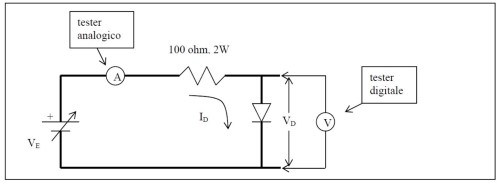
\includegraphics[width=\linewidth]{diodo.jpg}
    \caption{Schema di montaggio del diodo}
    \label{figura1}
\end{figure}
~
Il sistema così montato ci permette di misurare i valori sperimentali della tensione del diodo e della corrente all'interno del diodo perturbando il minimo possibile il sistema. Per eseguire l'esperimento si è scelto di misurare la tensione in funzione della corrente; la legge di riferimento è l'equazione 1. Per l'incertezza da attribuire al singolo dato si è utilizzato l'un percento del fondo scala del'amperometro per la corrente, mentre il 0.5 per cento del fondo scala per la tensione.

\section{Procedimento sperimentale:}
Sperimentalmente si è proceduto facendo l'ipotesi che la corrente di saturazione I$_{0}$ abbia un valore di 10$^{-12}$ Ampere, se eventualmente dovesse risultare uno shift tra i dati sperimentali e quelli teorici, si procederà a cambiare il valore fino a quando la curva teorica e quella sperimentale non si sovrappongono. I dati raccolti sono riportati nella Table 1.
~
\section{Analisi dati:}
Possiamo osservare che, nonostante ci sia una prima regione dove la curva teorica e quella sperimentale si sovrappongono per 3*10$^{-12}$ Ampere, c'è una regione dove i due grafici differiscono di molto, infatti quello sperimentale ha un andamento rettilineo, Figure 2.
~
\begin{figure}[h!]
    \centering
    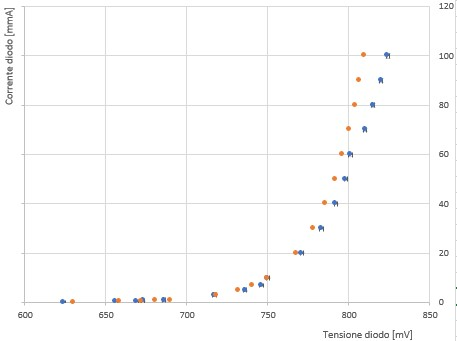
\includegraphics[width=\linewidth]{Confronto sperimentale e teorico.jpg}
    \caption{In arancione i punti teorici, in blu quelli sperimentali, si può osservare che dopo la regione esponenziale c'è una grande discrepanza}
    \label{figura1}
\end{figure}
~
Questo fenomeno può  essere spiegato semplicemente tenendo conto del fatto che il diodo presenta una resistenza ohmica, il cui contributo non è considerato nella legge di Shockley. Per valutare il valore di questa resistenza ohmica plottiamo un grafico V-I usando come tensioni la differenza tra tensione teorica e sperimentale da un certo valore di corrente in poi, questo plot è riportato in Figure 3 ed i dati usati in Table 2.
~
\begin{figure}[h!]
    \centering
    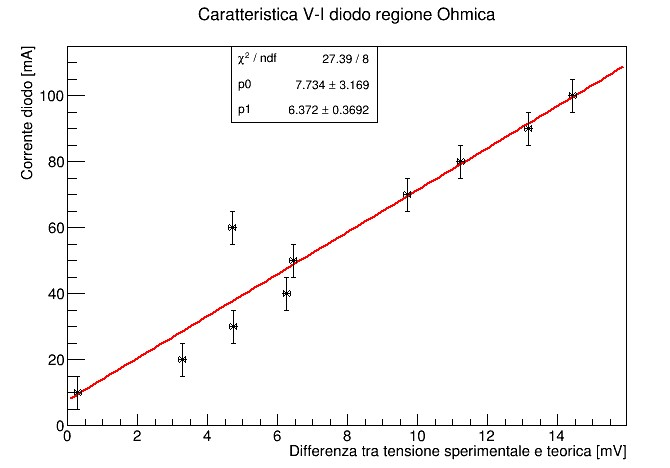
\includegraphics[width=\linewidth]{regione ohmica diodo.jpg}
    \caption{Plot V-I della regione ohmica del diodo}
    \label{figura1}
\end{figure}
~
Facendo così dal fit possiamo ottenere il valore della resistenza come:
\begin{equation}
    R_d=1/a
\end{equation}
dove con R$_{d}$ intendiamo la resistenza del diodo e con a intendiamo il coefficente angolare della retta ottenuta dal fit. Facendo così, possiamo utilizzare un nuovo valore di tensione:
\begin{equation}
    V'_d=V_d+I_d*R_d
\end{equation}
e quindi usare la tensione corretta ottenuta nella (3) nella equazione (1) e quindi plottare il grafico Figure 4. I dati usati provengono dalla Table 3.
~
\begin{figure}[h!]
    \centering
    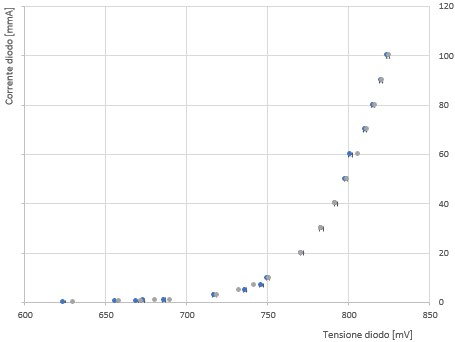
\includegraphics[width=\linewidth]{nuova teoria.jpg}
    \caption{con la correzione proveniente dal considerare il comportamento ohmico abbiamo un fit praticamente perfetto}
    \label{figura1}
\end{figure}
~
\section{Presentazione risultati e conclusioni:}
Come si può osservare dai grafici, senza tener conto del comportamento ohmico, con la legge di Shockley si può fittare la regione bassa dove abbiamo l'effetto dovuto alle caratteristiche intrinseche del diodo, con la correzione della regione ohmica possiamo fittare tutto il grafico e quindi possiamo concludere che la legge di Shockley è un ottimo modello per questa componente elettronica.
~
\section{Appendice:}
Tabelle di riferimento per i grafici:
~
\begin{table}[h!]
  \begin{center}
   \begin{tabular}{|c|c|c|c|c|c|c|}
      Ids[mA]&fsI[mA]&uIds[mA]&Vds[mV]&fsV[V]&uVds[mV]&Vdt[mV] \\
      0.10&5&0.05&624&2&10&629\\
      0.30&5&0.05&656&2&10&659\\
      0.50&5&0.05&669&2&10&672\\
      0.70&5&0.05&673&2&10&681\\
      1.00&5&0.05&686&2&10&690\\
      3.00&5&0.05&717&2&10&718\\
      5.00&50&0.50&736&2&10&732\\
      7.00&50&0.50&746&2&10&740\\
      10.00&500&5.00&750&2&10&751\\
      20.00&500&5.00&771&2&10&750\\
      30.00&500&5.00&783&2&10&778\\
      40.00&500&5.00&792&2&10&786\\
      50.00&500&5.00&798&2&10&791\\
      60.00&500&5.00&801&2&10&796\\
      70.00&500&5.00&810&2&10&800\\
      80.00&500&5.00&815&2&10&804\\
      90.00&500&5.00&820&2&10&807\\
      100.00&500&5.00&824&2&10&810
       \end{tabular}
  \caption{Tabella associata al primo grafico}
  \end{center}
\end{table} 
~
\begin{table}[h!]
  \begin{center}
   \begin{tabular}{|c|c|c|c|c|c|c|}
      Ids[mA]&fsI[mA]&uIds[mA]&diff.[mV]&uV[mV]\\
      10.00&500&5.00&0.29&0.10\\
      20.00&500&5.00&3.27&0.10\\
      30.00&500&5.00&4.73&0.10\\
      40.00&500&5.00&6.25&0.10\\
      50.00&500&5.00&6.44&0.10\\
      60.00&500&5.00&4.70&0.10\\
      70.00&500&5.00&9.70&0.10\\
      80.00&500&5.00&11.22&0.10\\
      90.00&500&5.00&13.16&0.10\\
      100.00&500&5.00&14.42&0.10
       \end{tabular}
  \caption{Tabella associata al secondo grafico}
  \end{center}
\end{table} 
~
\begin{table}[]
  \begin{center}
   \begin{tabular}{|c|c|c|c|c|c|c|}
      Ids[mA]&fsI[mA]&uIds[mA]&Vds[mV]&fsV[V]&uVds[mV]&V'dt[mV] \\
      0.10&5&0.05&624&2&10&629\\
      0.30&5&0.05&656&2&10&659\\
      0.50&5&0.05&669&2&10&672\\
      0.70&5&0.05&673&2&10&681\\
      1.00&5&0.05&686&2&10&690\\
      3.00&5&0.05&717&2&10&718\\
      5.00&50&0.50&736&2&10&732\\
      7.00&50&0.50&746&2&10&742\\
      10.00&500&5.00&750&2&10&751\\
      20.00&500&5.00&771&2&10&771\\
      30.00&500&5.00&783&2&10&783\\
      40.00&500&5.00&792&2&10&792\\
      50.00&500&5.00&798&2&10&800\\
      60.00&500&5.00&801&2&10&806\\
      70.00&500&5.00&810&2&10&812\\
      80.00&500&5.00&815&2&10&817\\
      90.00&500&5.00&820&2&10&821\\
      100.00&500&5.00&824&2&10&826
       \end{tabular}
  \caption{Tabella associata al terzo grafico}
  \end{center}
\end{table} 

\end{document}